\section{Preparation}\label{sec:prep}
Before the data can be further processed and used, some basic preparation
must be done to normalise the data.
This section discusses the transformative steps and the end representation that
the program will work with from the initial state until classification.

\subsection{Resampling}
Because the source recordings vary in format, we normalise these to the following
format:
\begin{itemize}[noitemsep]
  \item \textbf{Format:} Raw WAV
  \item \textbf{Audio channels:} 1
  \item \textbf{Bit depth:} 16-bits
  \item \textbf{Sample rate:} 22050 Hz
\end{itemize}

If a recording is found to have more than a single channel, all but the left
channel are discarded.
It is unclear whether discarding a channel is better than summing them.
While summing retains all information, it may also introduce further noise.
Conversely, it is allso possible for the left channel to have a worse signal to
noise ratio than the right.
The number of multi-channel recordings is low enough for this not to be much
of an issue.

Sample rates are reduced to lower the memory and processing demands of
analysing all 45 hours of audio.
Our image recognition approach holds greater importance to the general shape
of individual vocalisations in spectrograms, rather than high time-frequency
details.
Because of this, the sample rate reduction is found to have no significant
reductions in classification quality.

The recording duration is left unaltered, so durations may differ from sample to
sample.

The FFmpeg \parencite{ffmpeg} program is used to convert all source material.
We have written a shell script to make this procedure fully automatic, executable
when new recordings have been sourced.


\subsection{Spectrogram Representation}
A spectrogram is a visualisation of a sound as energy in the frequency spectrum
in function of time.
This allows us to intuitively visualise the shape of a sound as a 2d image.
Figure~\ref{fig:sgram_pcm} shows how the spectrogram representation retains
amplitude information from a waveform, while exposing the frequency composition
of the waveform.

\begin{figure}[!htb]
  \centering
  \begin{subfigure}[b]{1.0\textwidth}
    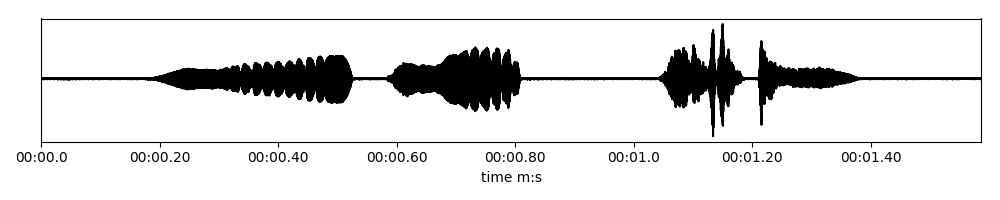
\includegraphics[width=1.0\textwidth]{pcm}
    \caption{}
  \end{subfigure}
  \begin{subfigure}[b]{1.0\textwidth}
    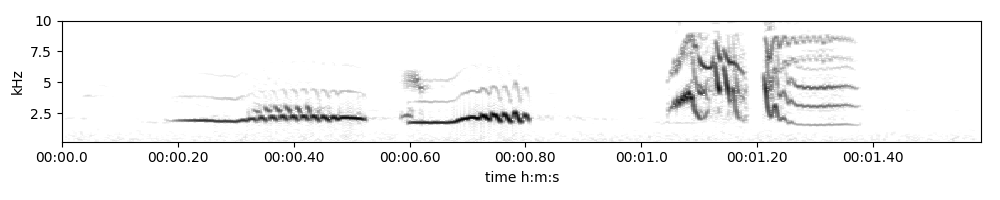
\includegraphics[width=1.0\textwidth]{sgram}
    \caption{}
  \end{subfigure}
  \caption{Waveform (a) and corresponding spectrogram (b) of a bird 1 recording}
  \label{fig:sgram_pcm}
\end{figure}

Our image recognition approach makes use of this spectrographic representation.

Spectrogram construction is performed for all recordings.
This is performed sequentially and immediately stored on disk.
The audio is first loaded as raw pulse-code modulation (PCM).
The windowed fast fourier transform (FFT) method is then used to generate a
spectrogram from the PCM.

Modern hardware handles FFT computations very well, making this stage very quick.
The Matplotlib \parencite{Hunter:2007} |specgram| function is used to generate
spectrograms.

The following parameters are used during spectrogram construction:
\begin{itemize}
  \item \textbf{NFFT}: 512.\\
   Defines the number of PCM data points used in each chunk.
  \item \textbf{Window}: Hann window of 512 points.\\
    Windowing is used to merge overlapping chunks.
  \item \textbf{Overlap}: 75\%.\\
    Overlap defines the number of points overlapping between chunks.
\end{itemize}

Spectrograms are converted to monochrome to simplify operations in the stages
that follow.
This does not reduce the information present in the spectrogram.

Frequencies above 10000Hz and below 100Hz are removed from the spectrograms as
these are less likely to contain relevant vocalisations \parencite{aab}.
These cuts will result in a reduction of baseline noise, as a lot of this falls
under 100 Hz.
